This section provides an example scenario of the communication protocol in action within a simplified abstracted architecture. For demonstration purposes, the underlying details of the hardware are omitted and only the utilization of the protocol itself is examined.

Figure!\ref{fig:frames} shows a series of frames segmented within PDP. For the purposes of this example, assume a system utilizing a single scene generator, compositor, and IRLED array. Assume also the average intensity of each region of a frame is computed during operation. The highlighted segments indicate a large change in intensity occurring within the region from frame to frame. Suppose that frames are generated at 4 times the rate of an external synchronization pulse. During operation within PDP, segments with a large change in intensity require higher frame-rate to reflect the fast frequency changes in intensity. The PDP protocol would be utilized to send these regions at a much higher frame rate than the slowly changing segments. Each segment would be sent using a region packet, one after another. Once sent, the remaining time would be utilized by a compositor to send the slower changing data at a much slower rate. In this particular example, the fast data for the frames could be sent at a rate much higher than that of the slowly changing segments; only updating the other segments once the fast moving data in all frames is sent. Once all data is sent, an external synchronization pulse from a sensor would then be utilized to indicate the data has been captured and a corresponding trigger packet sent from the compositor to scene generator to indicate that more frames be generated. The same procedure would then continue for the next set of frames.

\begin{figure}
    \centering
        \centering
        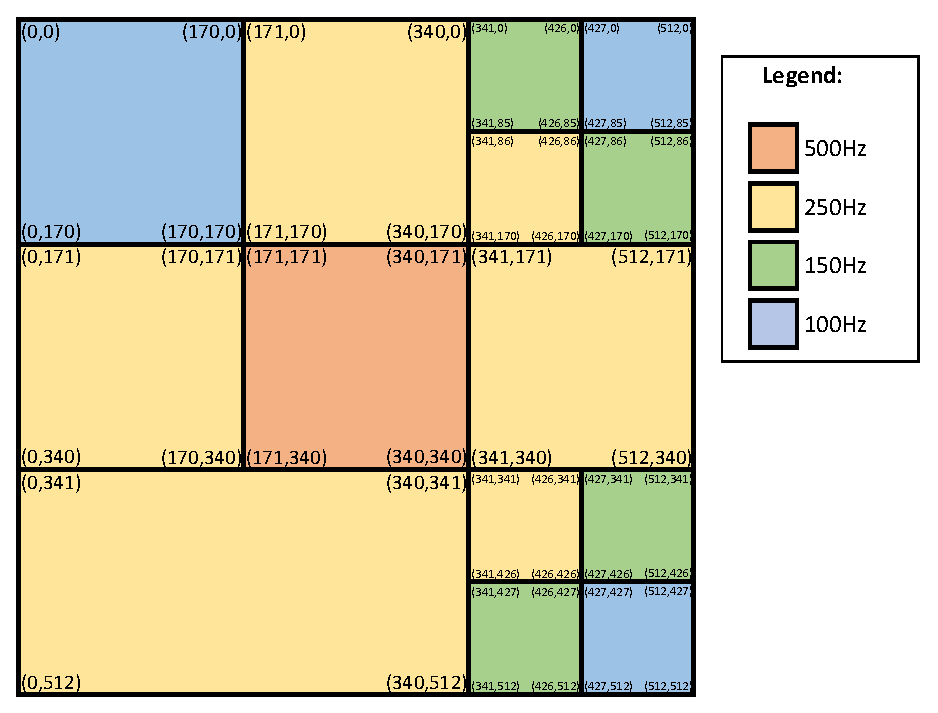
\includegraphics[width=1.0\textwidth]{fig/variable_display.pdf}
        \caption{Dynamic frame rate display with multiple regions updating at different frame rates}
        \label{fig:variable_display}
\end{figure}

\begin{figure}
        \centering
        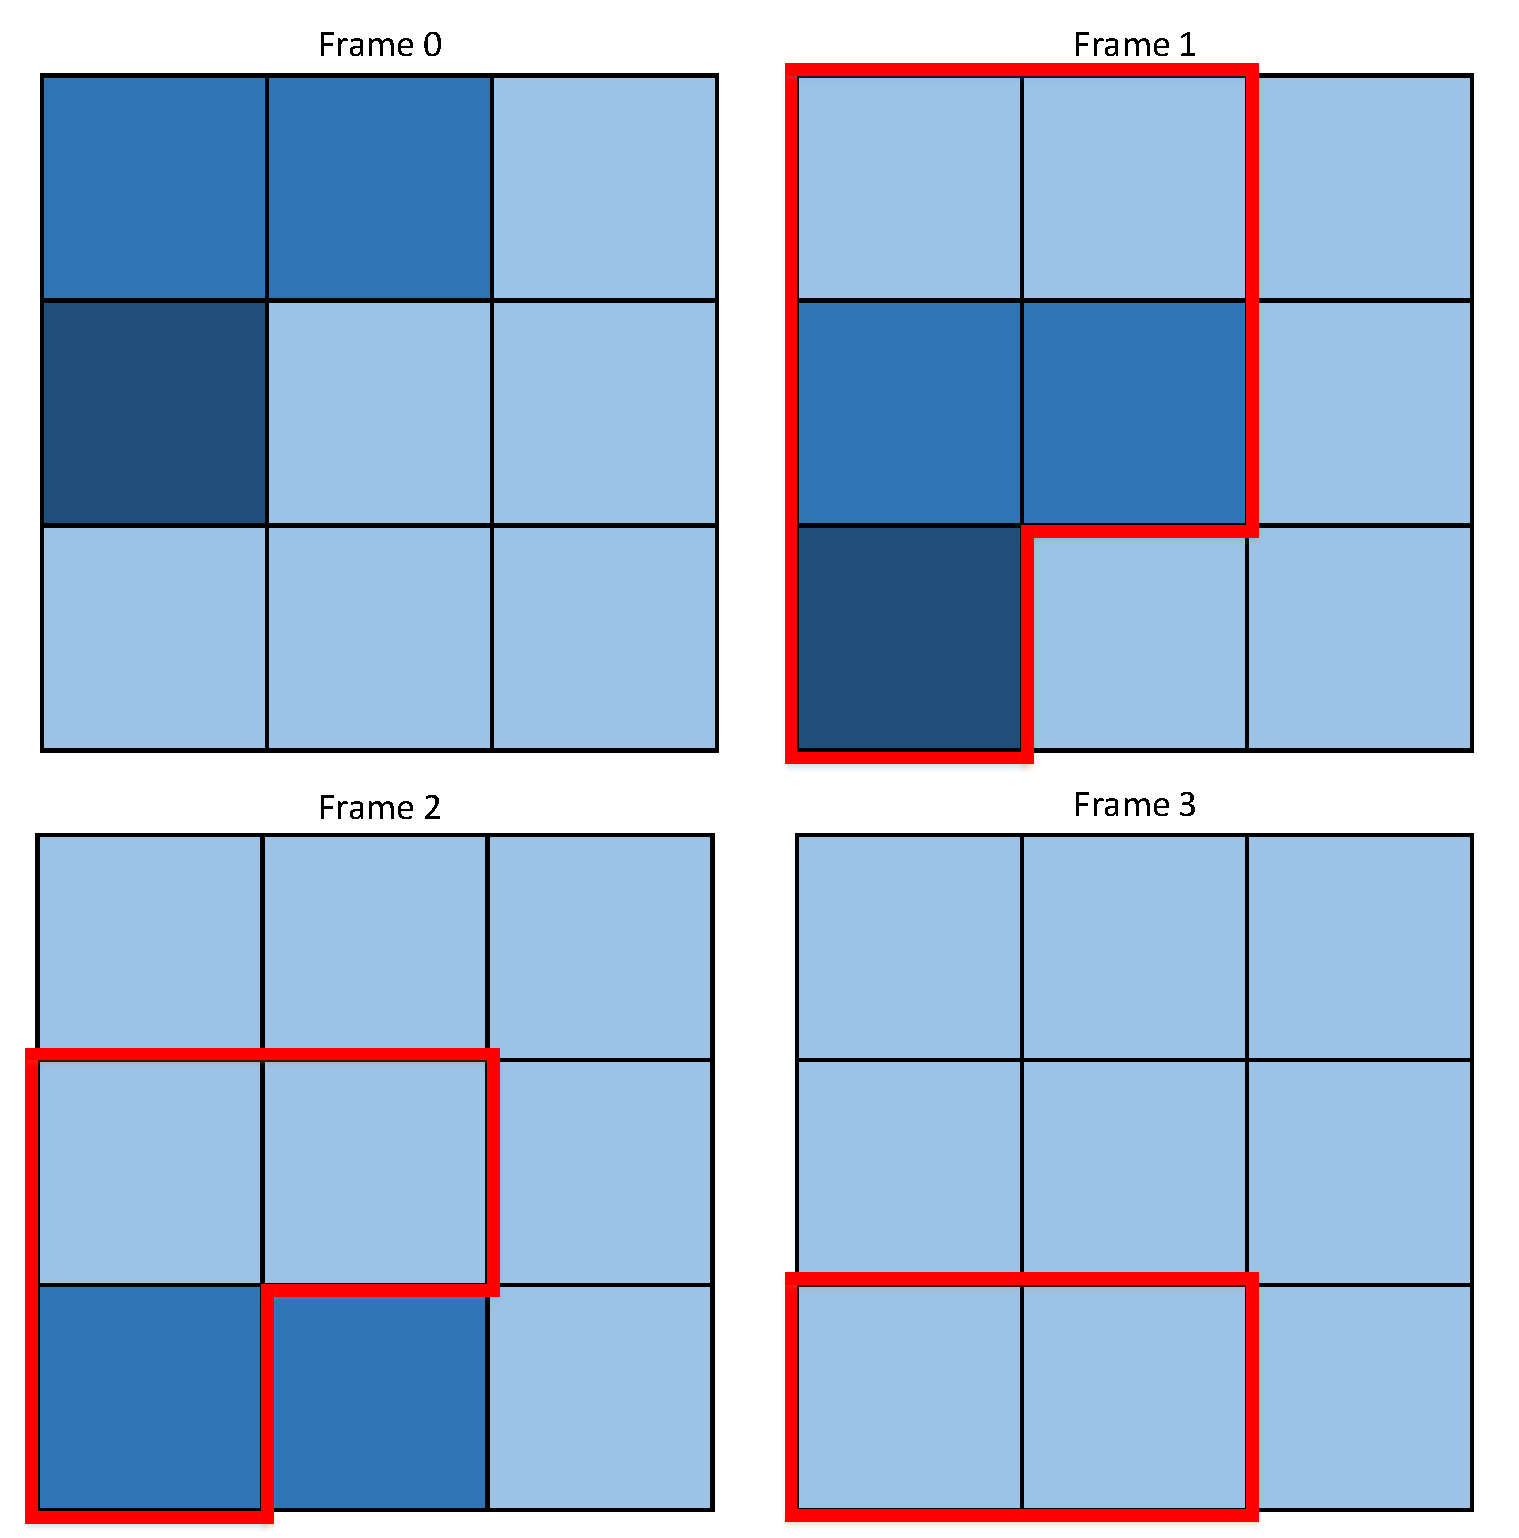
\includegraphics[width=1.0\textwidth]{fig/frames.pdf}
        \caption{Example display of frames within PDP. Each box indicates an average intensity for the given region}
        \label{fig:frames}
\end{figure}

In a real system, frames would be segmented more finely than in this example, allowing for small segments to be dynamically transmitted when needed. This would then give the ability for fast changing data to update at rates far greater than a static fixed frame rate display would be capable of doing under the same hardware considerations with limited bandwidth. Secondly, as discussed briefly above, this would give the analog portions of a display more time to settle thereby improving display fidelity. In more detail, the analog portions of a display are time constrained by the number of pixels that need to be addressed in a given time in fixed frame rate systems. By de-prioritizing slow changing data, these segments no longer need to be addressed at the same rate as the higher changing data in the display, allowing for more time for the high frame rate pixels to settle if needed.
